% Copyright (c) 2014,2016 Casper Ti. Vector
% Public domain.

\chapter{研究背景和目标} \label{chap:related}
\section{高速缓存的相关概念}
在本节中,我们将列举并解释在本文中出现的与高速缓存相关的一些重要概念。

\textbf{多级缓存}

因为内存访问的延迟较高,为了弥补CPU与内存之间的速度差异,现代计算机通常都采用了层
次化的高速缓存架构,我们称之为多级缓存(Multi-level Cache)。按照缓存距离CPU 的远近,依次将其称为L1、L2、L3 等。特别的,我们将体系结构上最远离CPU、存取速度最慢的那一级称为底层缓存(Last-Level Cache,LLC),其余的统称为高层缓存(Higher Level Cache)。在多核处理器中,每个处理器核(Core)通常具有各自独立的高层缓存,我们将它们称为核的私有缓存(Private Cache)。底层缓存却通常被多个核(甚至所有核)所共享,我们称其为共享缓存(Shared Cache)。这种设计既有助于在一定程度上保证核与核之间的隔离,同时又能使各个核在底层缓存上进行高效的数据交换,并简化处理器的硬件复杂度。

在多级缓存中,如果某级缓存所存储的数据同时存在于其下一级缓存中,我们就将这下一级缓存称为包含型缓存(Inclusive Cache)。反之,如果在同一时刻相邻两级缓存中没有重复的数据单元,我们就将较低的那级缓存称为排除型缓存(Exclusive Cache)。尽管包含型缓存造成了一定的空间浪费,但却有助于提高缓存同步(Cache Coherence)时的性能。这是因为如果发现要同步的数据不在该缓存中,我们就没有必要把同步操作再向上层传递。而且,对于共享的包含型缓存,我们还可以在其缓存单元中记录该数据还存放在哪些私有缓存中,而避免向所有上层缓存发出请求。所以,目前的商用处理器多采用包含型缓存的设计。

\begin{figure}[htbp] 
    \centering
    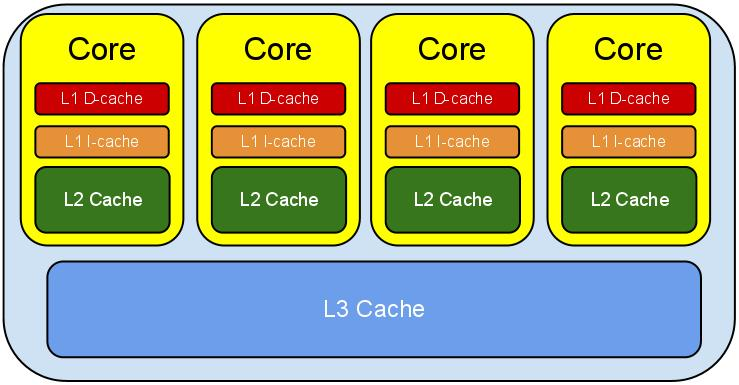
\includegraphics[width=0.7\linewidth]{figures/CacheHierarchy.jpg}
    \caption{多级缓存的示例}
    \label{fig:cache_hierarchy}
\end{figure}

如图\ref{fig:cache_hierarchy}所示是一个典型的多级缓存设计,英特尔近年的微处理器架构,包括都Sandy Bridge、Haswell、Skylake,都采用了这一设计。每个处理器核拥有两层独立的私有缓存,第一层私有缓存包括L1 D-cache和L2 I-Cache,分别负责数据和指令缓存;第二层私有缓存L2 Cache。L1、L2缓存每个核都有且独占。底层缓存LLC,也可以被称为L3 Cache,为所有核所共享。L1、L2的缓存大小通常在KB级,L3/LLC的大小通常在MB级,高端处理器中可达数十MB。


\textbf{相联度}

缓存中一个最小的存储单元称为缓存块(Cache Line)。缓存的相联度(Associativity)决定了某个内存地址的数据能存放在哪些缓存块中。

相联度为1的缓存称为直接映射缓存(Direct Mapped Cache)(图\ref{fig:cache_asso}(a))。对于直接映射缓存,硬件会将内存地址的一部分作为索引,将其对应到一个唯一的缓存块。因此,每块内存数据都只能存放在一个特定的缓存块中,而如果两个内存地址的索引部分相同,就将导致冲突(Conflict)。

如果缓存的相联度和缓存块的总数相同, 则称之为全相联缓存(Full Associative Cache(图\ref{fig:cache_asso}(b))。在全相联缓存中,一个内存地址能缓存在任何一个缓存块中,硬件通过全相联比较器确定该内存地址被缓存的位置。全相联缓存能够使缓存空间得到更有效的利用,但却需要极大的硬件复杂度。

组相联缓存(Set Associative Cache)是以上两种类型的混合(图\ref{fig:cache_asso}(c))。它按照相联度将缓存块平均分为若干缓存组(Set),同组内的各缓存块称为路(Way),路的数目就是缓存的相联度。分配缓存时,硬件首先根据内存地址的一部分确定该数据所对应的缓存组,数据可以缓存在该组内的任何一个缓存块中。硬件设计人员可以通过控制相联度,在冲突失效率及硬件复杂度之间做出权衡。现代处理器多采用这种设计。

\begin{figure}[htbp] 
    \centering
    \begin{subfigure}[b]{0.24\linewidth}
        \centering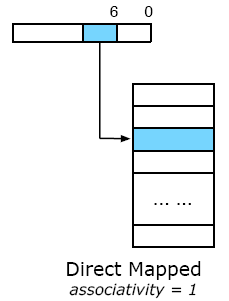
\includegraphics[width=0.9\linewidth]{figures/CacheAsso1.png}
        \caption{直接映射}
    \end{subfigure}%
    \begin{subfigure}[b]{0.24\linewidth}
        \centering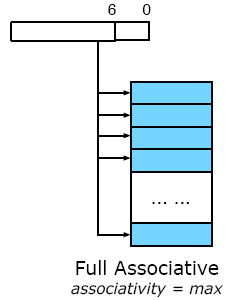
\includegraphics[width=0.9\linewidth]{figures/CacheAsso2.png}
        \caption{全相联}
    \end{subfigure}%
    \begin{subfigure}[b]{0.52\linewidth}
        \centering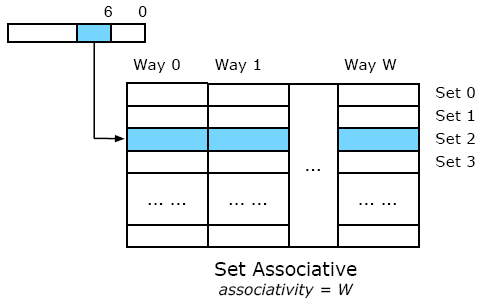
\includegraphics[width=0.9\linewidth]{figures/CacheAsso3.png}
        \caption{组相联}
    \end{subfigure}
    \caption{缓存的相联度}
    \label{fig:cache_asso}
\end{figure}

\textbf{管理策略}

为了管理全相联缓存和组相联缓存中自由的缓存空间,硬件通常以队列的逻辑形式来组织这些缓存块。当缓存失效(Cache Miss)时,新数据将插入队列的什么位置取决于缓存的插入策略(Instertion Policy)。当要缓存的内容超过缓存容量时,硬件就会按照某种策略从队列中淘汰一个缓存块,这个策略称为替换策略(Replacement Policy)。当缓存命中(Cache Hit)时,如何调整命中的缓存块在队列中的位置取决于缓存的晋升策略(Promotion Policy)。

由于局部性原理,最近最少使用(Least Recently Used,LRU)是最为被广泛使用的缓存队列组织形式。在LRU 队列中,我们将队首的位置称为MRU(Most Recently Used),将队尾的位置称为LRU。那么其管理策略就可以概括为:新数据插入到MRU 的位置,从LRU 的位置淘汰数据,命中的数据将晋升到MRU的位置。

由于程序的数据访问在时间和空间上会有局部性的特性,即如果一个信息项正在被访问,那么在近期它很可能还会被再次访问;以及在最近的将来将用到的信息很可能与现在正在使用的信息在空间地址上是临近的。所以LRU策略可以提供较好的缓存管理效率。严格的LRU在实现上比较困难,且会带来较大的额外开销,所以现代处理器多采用近似LRU的管理策略。

\section{缓存划分的相关研究}
在LRU策略下的共享缓存LLC中,不管访问来源与哪个核都被一视同仁,也就是说所有核在竞争使用LLC。然而,竞争的结果往往不是效率最高的结果。因为某些高污染程序,比如流媒体应用,往往会占据大量的缓存资源,从而导致同时运行的其他程序因为没有足够的缓存而性能下降。如何高效地管理和优化共享缓存是学术界非常关心的一个问题。优化共享缓存的一个关键点就是通过缓存的划分,来改善系统的整体性能。我们广泛调研了关于缓存划分技术的相关研究,将其归纳为硬件技术和软件技术两大类。

\textbf{硬件技术}

基于硬件的研究主要通过改良缓存硬件、优化缓存管理策略等方法来完成缓存的优化。

Suh等首先提出了动态缓存划分的思想来优化共享缓存的利用率~\parencite{suh2002new,suh2004dynamic,suh2014analytical}。他们采用了一种软硬件结合的方法,首先由修改过的硬件动态构造出一个失效率曲线,然后操作系统利用该曲线求出使得总失效率最低的一种划分方案,最后再由CPU通过修改缓存替换策略完成缓存分割。这种方法带来了很大的硬件开销。

Qureshi等对上述方法加以改进~\parencite{qureshi2006utility,qureshi2007adaptive},他们将增加单位缓存后某个程序减少的失效数称为效用(Utility),并实现了以最大化全局效用为目标的缓存划分方法。其主要优化包括:为每个核构造单独的失效率曲线图,以提高决策的准确度、用组采样(Set Sampling)来降低硬件开销,以及优化寻找最优划分的贪心算法。试验表明,该方法能够用较小的硬件开销实现平均情况下11\%的性能提升。

Rafique等给出了一种通用的、让操作系统自由控制缓存配额的软硬件接口
~\parencite{rafique2006architectural}。他们设计了该接口的体系结构支持,并在模拟器上评测了若干策略。他们认为,这种策略与机制相分离的方法具有更强的适用性。

Srikantaiah等提出了一种自适应组独占(Adaptive Set Pinning)的方法~\parencite{srikantaiah2009sharp}。它能自动根据需要,将某些缓存组分配给某个处理器核独占使用一段时间,从而同时减少核与核间由于同步操作导致的缓存失效,以及处理器核自身由于容量限制或地
址冲突导致的缓存失效。

Xie 等提出了一种称为PIPP的缓存“伪划分”技术~\parencite{xie2009pipp}。他们首先用Qureshi 的方法得到一个最优的划分方案,再通过调整缓存的插入策略和晋升策略,使缓存的分配动态平衡在想要的划分比例。他们的实验结果表明,这种方法避免了刚性划分所引起的缓存空间利用不当,能够综合Qureshi工作的优点。

此外,还有一些研究针对不同的优化目标。Iyer等提出了基于服务质量(Quality of Service, QoS)的优化模型。针对多核平台下任务多样性的新趋势,QoS 存储架构能够根据应用的优先级,可控地分配缓存空间和内存带宽等资源~\parencite{iyer2004cqos}。Kim 等提出了以性能公平性(Fairness)为目标的共享缓存管理策略~\parencite{kim2004fair}。Hsu等总结了基于性能、服务质量以及公平性这三方面的优化目标~\parencite{hsu2006communist},并提出相应的优化策略。

上述这些研究,虽然在优化目标、策略及算法上有所不同,但实现缓存划分的方式都是基于路的划分(Way Partitioning)。路划分技术是将缓存的路(Way)分配给各个核,它的最小划分单位为一个缓存路。之所以路划分技术被广泛使用是因为其设计简单,不需要很复杂的硬件修改。但是它的不足之处在于分配的粒度较粗,一个路往往会有很多缓存块,这在核数较多时会显得力不从心,因为最优划分很可能会且在一个路的中间。对于一个处理器而言,缓存的路数在设计之处就已经确定,而且数目不会太多,当核数增加时,分配的灵活性将会大大下降。当核数等于路数时,每个核有且只能被分配一个路,这就彻底失去了灵活性,只能起到隔离的效果。

一些研究试图改进路划分技术,提高分配粒度。Chang等提出了称为CCP共享缓存的技术~\parencite{chang2006cooperative,chang2014cooperative}。这种方法从时间和空间两个维度上分配共享的缓存资源。它可以通过控制处理器核使用某个缓存分区的时间片长短来保证公平性,并通过伸缩每个缓存分区的大小来控制服务质量。通过时间共享来细化划分粒度。Manikantan提出了PriSM通过精确地控制缓存失效概率来细化分配粒度~\parencite{manikantan2012probabilistic}。还有一些研究抛弃了路划分,采用更加复杂的硬件设计来实现细粒度缓存分配~\parencite{sanchez2011vantage}。

所有的硬件研究因为涉及到硬件修改,所以基本都是在模拟器中进行。

\textbf{软件技术}

软件方面主要依赖于“页面着色”(Page Coloring)这一技术。Lin等首先提出了“页面着色”技术~\parencite{lin2008gaining},在Linux 操作系统上实现了无需硬件支持的缓存分区,它们提出了一种按照失效率和敏感度对应用程序使用缓存的特征进行分类方法,并利用该方法设计了若干组基准程序,评估了页面着色方法对他们的效果。之后多个学者对这一技术进行了更深入的研究和应用~\parencite{zhang2009towards,soares2008reducing,tam2007managing,azimi2009enhancing,lu2009soft}。

页面着色的基本原理是通过操作系统控制页面到缓存块的映射,从而限制缓存被分配的区域。这种技术可以在真实系统上通过软件实现,而且原则上来说可以将分配粒度细化到一个缓存块。然而,目前处理器纷纷采用哈希算法映射物理地址到缓存块,而不是过去的一一对应。在不知道哈希函数的情况下,就无法通过页面着色来控制缓存块的分配。所以现在页面着色技术已经不再适用。

\section{英特尔高速缓存分配技术}
英特尔在2016年发布的第四代至强处理器产品家族中全线引入了资源调配技术(RDT),高速缓存分配技术(CAT)是其中重要的组成部分。高速缓存分配技术首次在商用处理器上实现了对共享缓存(LLC)容量的管理。通过CAT技术,我们可以在软件层面为每个核分配可使用的缓存资源。下面我们简要介绍CAT的使用方法。

CAT通过一个被称为CLOS(Class of Service)的单元来控制缓存的分配。每个CLOS包含一个CBM(Capacity Bitmask)的容量掩码,代表该CLOS可以使用哪些缓存。CBM是由一串连续的1构成01串,1代表当前位这一路的缓存可以被适用,0代表不能被使用。将处理器核与某个CLOS绑定,该核就只能占用被CLOS中的CBM所指定的缓存。

图 \ref{fig:CLOS}是一个CLOS与CBM的例子。CLOS[0]分配有第19到第16路的缓存,CLOS[1]分配有第15到第12路缓存,CLOS[2]分配有11到第6路缓存,这一部分与CLOS[3]发生了重叠。一个核与某个CLOS绑定后就会受到其限制了。

\begin{figure}[htbp] 
    \centering
    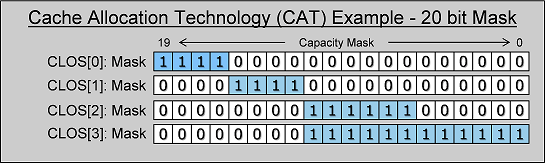
\includegraphics[width=0.7\linewidth]{figures/CLOS.png}
    \caption{CLOS与CBM的示例}
    \label{fig:CLOS}
\end{figure}

CAT借鉴了前人的研究成果,采用了路划分(Way Partitioning)技术这一设计。前人在模拟器中可以调整缓存路数,然而真实处理器中的路数是固定的。CAT可分配的路数非常有限,在最高端的CPU中仅有20路可供分配,每一路高达几兆字节的缓存空间,所以说CAT的分配粒度很粗。

此外CAT技术与以往的技术有两点很大的不同:
\begin{itemize}
\item 分配必须是连续的。CBM必须包含连续的1,例如,“0111”是一个有效的分配,而“1011”则不行。
\item 分配间允许重叠。例如,可以把“1110”分配给一个核,“0111”分配给另外一个核,中间两路缓存两个核所共享。
\end{itemize}

这两个特点意味着在CAT中分配的位置也需要被考虑。以往的研究通常只需要考虑分配“多少”缓存,因为分配不一定要连续而且不会重叠。而CAT中因为连续的要求和允许重叠,所以分配在“哪里”也同样重要。

目前关于CAT的研究都集中在QoS方面~\parencite{lo2015heracles, herdrich2016cache, funaro2016ginseng}。它们主要通过提供给高优先级的程序足够的缓存资源来满足QoS要求,而让低优先级程序共享剩余的缓存。这种思路并不需要细粒度的缓存控制,所以CAT可以轻松胜任。

\section{研究目标}
随着处理器中的核数越来越多,共享缓存的竞争问题也愈发严重。目前,还没有一个可以在真实系统上可以运行的缓存优化框架,我们希望通过我们的努力实现这样一个框架的原型。我们称之为CAPS,它可以满足以下几个方面的要求:(1)\textbf{可以在真实系统中运行};(2)\textbf{实现细粒度分配控制};(3)\textbf{良好的可扩展性,在核数较多时依然有很好的适应性};(4)\textbf{具备灵活性,支持多种优化策略}。

共享缓存分配优化的步骤一般包含以下三步:
\begin{enumerate}
\item 预测。首先需要在任意分配情况下,对每个并发程序的性能进行预测和评估。性能参数包括失效率(Miss Rate)和周期指令数(IPC)等等。预测的指标用来为后面的决策提供参考依据。
\item 决策。根据预测的指标,和优化目标,做出一个分配决策。针对不同的优化目标,可能会采取不同的策略和算法。
\item 实施。将决策的分配付诸实践,让分配真正产生效果。
\end{enumerate}

若要在真实系统上实施分配,CAT技术是目前唯一的方法。所以CAPS必须倚仗于CAT作为最后实施分配的方法。而分配技术对前两个步骤,即预测和决策又有深远的影响,因为决策所得到的分配必须符合分配技术的要求,而预测又是为决策所服务。如上节所述,CAT技术要求分配必须连续以及有限的可分配资源都为实现细粒度、可扩展和灵活的分配优化带来了极大的困难。然而,CAT允许重叠这一特性却带来很大的操作空间。虽然重叠分配,尤其是部分重叠,为预测模型和分配决策带来了更大的挑战,但是我们通过研究探索,在CAPS中实现了一个全新的预测模型,以及一个基于模拟退火的决策算法,可以支持部分重叠下的CAT分配的性能预测和优化决策,让上述提出的四点目标得以满足。在下一章中,我们将首先介绍CAPS预测模型。

